\subsection{SODA : The State-of-the-Art Tool\label{SODA}}

%As mentioned earlier, the only approach currently available is SODA~\cite{Moha12-ICSOC-SOASpecificationDetection, Nayrolles12-ICSOC-SODA}. 
SODA relies on a rule-based language that enables antipatterns specification using a set of metrics. A generic process then turns the specification into detection algorithms. The three main steps of the processing are as follows (see Figure~\ref{fig:The-SODA-approach}):

\begin{figure*}
\framebox{\begin{minipage}[t]{1pt + 2\columnwidth}%
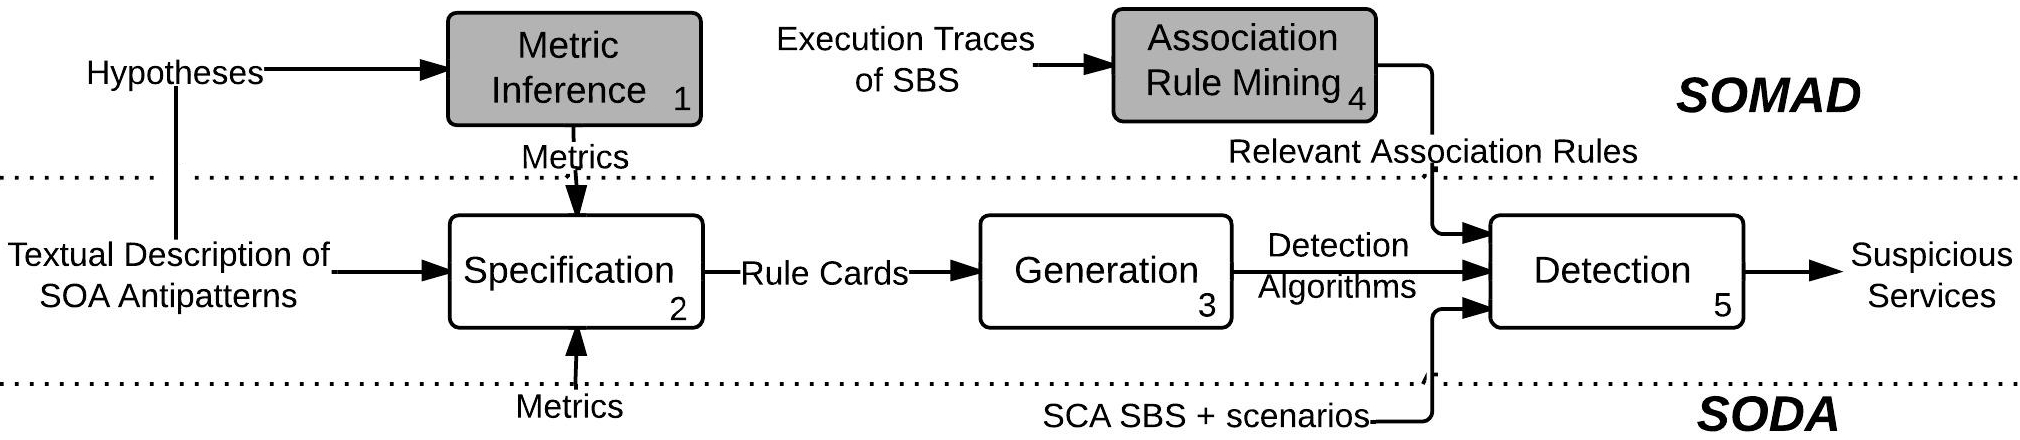
\includegraphics[scale=0.25]{media/SODA.png}%
\end{minipage}}
\caption{\label{fig:The-SODA-approach}SODA and SOMAD approaches: Grey boxes depict new steps in SOMAD w.r.t. to SODA (white boxes).}
\end{figure*}

\emph{Specification of SOA Antipatterns}: Relevant properties of SOA antipatterns are identified, which essentially correspond to metrics such as cohesion, coupling, number of methods, response time and availability. These properties compose to a base vocabulary of a DSL: a rule-based language is used whereby each rule expresses tendencies in metric values. An antipattern is described by a set of rules combined into a \textit{rule card}.

\vspace{0.12cm}

\emph{Generation of Detection Algorithms}: Automatic generation of detection algorithms is performed by visiting models of rule cards specified during the previous step. The process is straightforward and ends up with a set of directly executable algorithms.
%The generation process relies on Java code templates that correspond to the detection algorithms. .

\vspace{0.12cm}

\emph{Detection of SOA Antipatterns}: The detection algorithms generated in the previous step are applied on the SBS of interest. This step allows the automatic detection of SOA antipatterns using a set of predefined scenarios to invoke service interfaces. At the end, services from the SBS suspected of being involved in an antipattern are identified.

\vspace{0.15cm}

Although efficient and precise, SODA is an intrusive approach because it requires a set of valid scenarios concretely invoking the interface methods of SBSs and its dynamic analysis involves SCA properties. 

%
%\textcolor{blue}{\emph{Step 1. Specify SOA antipatterns:} This step lies in identifying properties in SBSs relevant to SOA antipatterns. 
%To achieve the specification we perform a thorough domain analysis of SOA antipatterns by analyzing their definitions and specification in the literature to identify relevant properties. These properties are used as a base vocabulary (Cohesion, Coupling, ...) to a DSL, in the form of a rule-based language for specifying antipatterns.}
%
%\textcolor{blue}{\emph{Step 2. Generate detection algorithms: }In this step, detection algorithms are generated automatically from the specifications defined in the previous step. Using the previous specification and our DSL; we implemented the generations as a set of visitors on models of the antipatterns rule card (rule cards are combination of rules). These algorithms are directly executable.} 
%
%\textcolor{blue}{\emph{Step 3. Detection: }Detect automatically SOA antipatterns: The third step consists of applying, on the SBSs of interest, the detection algorithms generated in \emph{Step 2} to detect SOA antipatterns.}
